\section{Zeitmanagement}

\subsection{Zeitaufwand pro Person und Kategorie}
Die untenstehende Tabelle zeigt auf, wer wie viel Arbeit pro Kategorie aufgewendet hat.
\begin{figure}[H]
	\centering
	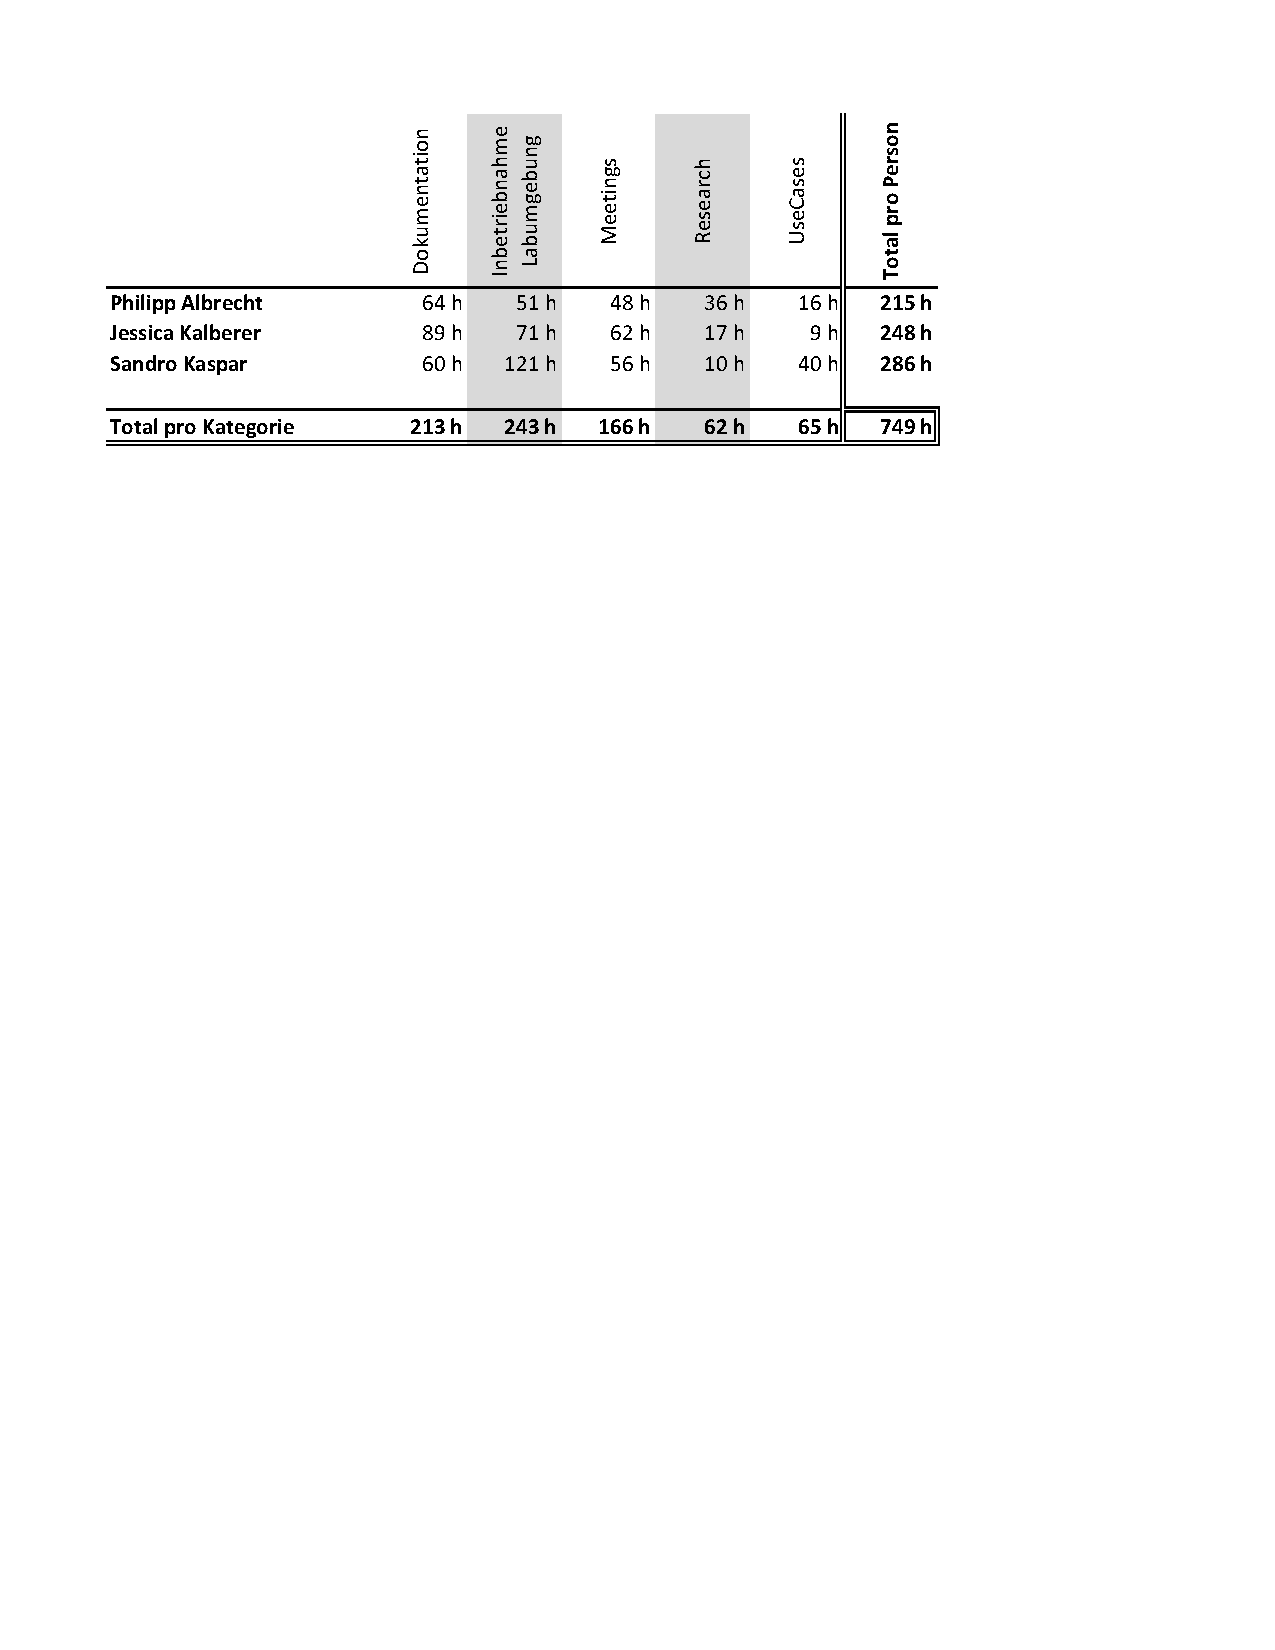
\includegraphics[]{img/zeitaufwand/zeitaufwand_pro_person.pdf}
	\caption{Zeitaufwand pro Person und Kategorie}	\label{fig:zeitmanagement-person-kategorie}
\end{figure} 

\subsection{Verteilung pro Kategorie}
Die nachfolgende Grafik beschreibt die Aufteilung der kompletten Arbeitsleistung in die einzelnen Kategorien.
\begin{figure}[H]
	\centering
	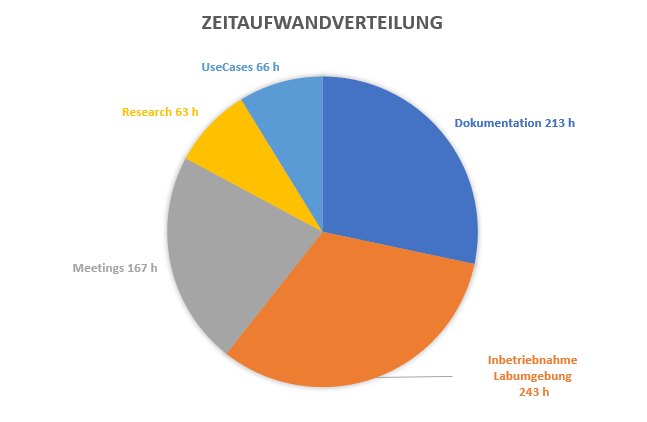
\includegraphics[width=15cm]{img/zeitaufwand/zeitaufwandverteilung.PNG}
	\caption{Prozentuale Verteilung nach Kategorie}
	\label{fig:zeitmanagement-kategorie}
\end{figure} 

\subsection{Zeitaufwand pro Woche}
Im nächsten Bild ist der Zeitaufwand pro Woche ersichtlich. Besonders hervorzuheben ist der Anstieg ab Woche 16, da zu diesem Zeitpunkt die Hardware eingetroffen ist.
\begin{figure}[H]
	\centering
	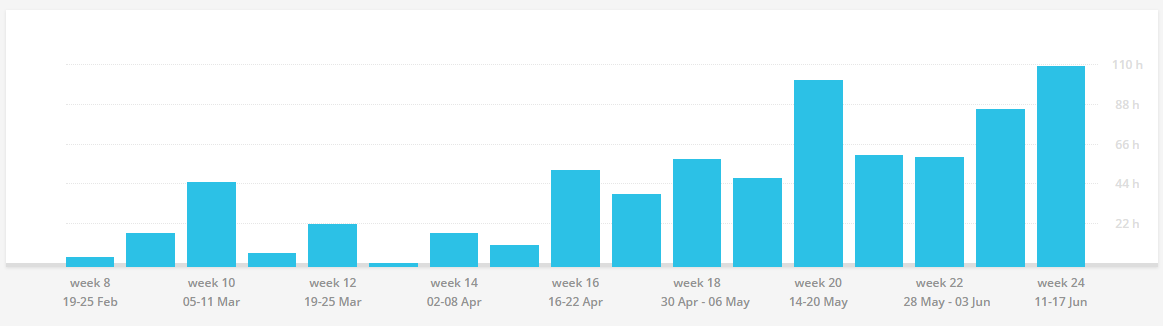
\includegraphics[width=16cm]{img/zeitaufwand/zeitaufwand_monat.PNG}
	\caption{Zeitaufwand pro Woche}
	\label{fig:zeitmanagement-zeit}
\end{figure} 